\documentclass[twocolumn,a4paper,dvipdfmx]{ieicejsp}
\usepackage[T1]{fontenc}
\usepackage{lmodern}
\usepackage{textcomp}
\usepackage{latexsym}
\usepackage{float}
\usepackage{graphicx}
\usepackage{amsmath, amssymb}
\usepackage{bm}
\usepackage{upgreek}
\usepackage{caption}
\usepackage{booktabs}
\usepackage{multirow}
\usepackage{tikz}
\usepackage{xcolor}
\usepackage{url}
\usetikzlibrary{positioning, arrows.meta}

\captionsetup{font=small}
\DeclareMathOperator*{\argmax}{arg\,max}
% 修正箇所を赤字で示すコマンド
\newcommand{\add}[1]{{\color{red}#1}}

\title{
    {\bf 物体領域検出とカテゴリアノテーションの分離に基づく，\\WordNetを用いた粒度可変物体アノテーション}
    {\normalsize \\ Adjustable-Granularity Object Annotation via Decoupled Region Detection and WordNet-Guided Category Annotation}
}
\author{
    著者名 \\ Author Name
}
\affliate{%
    所属機関名 \\
    Affiliation \\
}

\begin{document}
\maketitle

\begin{abstract}
本稿では，画像中の物体らしい領域を検出するタスクと，その領域に対応するカテゴリをアノテーションするタスクを明確に分離した物体アノテーション手法を提案する．
物体領域の検出にはカテゴリに依存しないDEtection TRansformer（DETR）を用いて1回の推論でバウンディングボックスを得る．
カテゴリのアノテーションには，各領域のクロップに対する視覚言語モデル（Vision-Language Model，VLM）のゼロショット分類を用いる．
両者が分離されているため，一度検出した領域に対して候補語彙集合を変更するだけでカテゴリのアノテーションを繰り返すことができる．
さらに，WordNetの上位語・下位語関係をたどることで，追加学習なしに「animal → dog → doberman」のような粒度可変のアノテーションを実現する．
COCO 2017 Validationの500枚を用いた評価により，以下を確認した．
第一に，ImageNetで学習した閉域の分類モデルに比べてContrastive Language-Image Pre-training（CLIP）は画像単位の単語推定精度が統計的に有意に高く，カテゴリのアノテーションにはオープンボキャブラリなVLMが必要である．
第二に，クラス非依存の位置検出精度において，DETRはOWL-ViTおよびGrounding DINOに劣らない．
第三に，提案パイプライン全体のカテゴリアノテーション精度はTop-1正解率0.604，Top-5正解率0.894であり，クロップを正方形にパディングしてVLMへ入力することでTop-1正解率が約0.08向上する．
第四に，WordNet階層の最初の細分化の段階で確信度が0.642から0.442へ大きく低下する．
また，下位語が1語しかない分岐が細分化の段階全体の約18\%で生じ，これが深い階層における見かけの確信度を押し上げていることを明らかにした．
さらに，COCOの80クラスで学習したYOLOと同一の語彙で比較し，80クラスの範囲内ではYOLOのTop-1正解率が0.98と提案手法を大きく上回るものの，その差は検出器ではなく分類器に起因すること，およびYOLOはCOCO外の物体をbirdやdog等の80クラス内の語でしかアノテーションできないことを示した．
加えて，深さ0のカテゴリをYOLOの予測とし，深さ1以降の細分化のみをVLMとWordNetで行うハイブリッド構成により，深さ0のTop-1正解率0.981を保ったまま，粒度可変のアノテーションの対象となるインスタンスを提案手法の1.65倍に増やせること，およびVLMの確信度が0.5以上の場合のみCOCO外の語に切り替えることで，\add{COCOの精度をほぼ損なわずに}，COCO外の物体の実画像にも対応できることを示した．
\add{さらに，別の500枚とLVISの細かい粒度の正解を用いて，これらの結論が別の画像でも成り立つこと，深さ0が正しくても深さ1の推定が正しいのは半数未満であること，および累積確信度による細分化の停止によって階層的適合率が0.594から0.801へ向上することを示した．}
COCOに含まれない語を主要な被写体とする実画像に対しても追加学習なしに正しくアノテーションできる一方，空を背景とした塔状の構造物ではDETRの検出自体が失敗することも確認した．
\end{abstract}

\noindent
{\bf キーワード：}オープンボキャブラリ物体アノテーション，DETR，視覚言語モデル，CLIP，WordNet，粒度可変アノテーション

\section{はじめに}
画像データセットに対する物体アノテーションは，画像中のどこに物体が存在するかという物体領域の判断と，その物体が何であるかというカテゴリの判断の2種類から構成される．
You Only Look Once（YOLO）\cite{ref_YOLO}やDETR\cite{ref_DETR}に代表される一般的な物体検出モデルは，これら2つの判断を単一のモデルに統合し，あらかじめ定めた固定のクラス集合に対して同時に学習する．
そのため，学習時に定めたクラス集合の範囲内では高精度な検出が可能である一方，学習後に新たなカテゴリを追加したり，カテゴリの粒度を変更したりする場合には，モデル自体の再学習が必要になる．

近年では，OWL-ViT\cite{ref_OWLViT}やGrounding DINO\cite{ref_GDINO}のように，カテゴリ名を自然言語のテキストクエリとして与えることで，固定のクラス集合に依存せずに物体を検出するオープンボキャブラリ物体検出モデルが提案されている．
しかし，これらのモデルも物体領域の検出とカテゴリの予測を単一のモデルの中で同時に行う．
そのため，例えば「動物」という粗いカテゴリで検出した物体を「犬」「猫」のようなより細かいカテゴリで改めて分類したい場合，候補カテゴリ集合を変更した上で検出処理そのものを再度実行する必要がある．

本研究では，物体領域の検出とカテゴリのアノテーションという2つの判断を明確に分離したアーキテクチャを提案する．
物体領域の検出には，カテゴリに依存しないバウンディングボックスを1回の推論で出力するDETRを用いる．
カテゴリのアノテーションには，検出済みの領域を切り出した画像（クロップ）に対し，VLMによるゼロショット分類を適用する．
両者が分離されているため，同一の検出結果に対して候補となる語彙集合を変更するだけで，検出処理を再実行することなくカテゴリのアノテーションを繰り返すことができる．
本研究はこの性質を利用し，WordNet\cite{ref_WordNet}の上位語・下位語関係をたどることで，追加学習を行わずに「animal → dog → doberman」のような粒度可変のアノテーションを実現する手法を提案する．

本稿の貢献は以下の4点である．
第一に，物体領域の検出とカテゴリのアノテーションを分離するアーキテクチャと，その分離を利用したWordNetによる粒度可変アノテーションの手法を提案する．
第二に，COCO 2017 Validationを用いた定量評価により，カテゴリのアノテーションにはオープンボキャブラリなVLMが必要であること，および物体領域の検出にDETRを用いることが位置検出精度の観点から妥当であることを示す．
さらに，閉域物体検出モデルであるYOLOと同一の語彙で比較し，提案手法の利点と限界を定量的に示す．
また，YOLOの予測を深さ0に用い，深さ1以降の細分化のみをVLMで行うハイブリッド構成を評価し，YOLOの精度と本手法の粒度可変性を両立できることを示す．
\add{さらに，閾値の選択に用いない別の画像と，WordNetのSynsetが付与されたLVISのアノテーションを用いて，深さ0の誤りの伝播と深さ1以降の推定の正誤を評価し，累積確信度による細分化の停止規則を提案する．}
第三に，提案パイプライン全体のカテゴリアノテーション精度を評価し，論文等で明示されることの少ないクロップの前処理と検出スコアの閾値が精度に大きく影響することを示す．
第四に，WordNet階層の各深さにおけるVLMの確信度を定量的に評価し，粒度を細かくするにつれて確信度が変化する傾向と，WordNetの生の階層構造を候補語彙として用いることに起因する限界を，下位語が1語しかない分岐の頻度を含めて明らかにする．

本稿の構成は以下のとおりである．
2章では関連研究について述べる．
3章では提案手法について述べる．
4章では実験条件と結果を示し，5章で考察を行う．
6章で本稿をまとめる．

\section{関連研究}
\subsection{閉域的な物体検出モデル}
YOLO\cite{ref_YOLO}やDETR\cite{ref_DETR}に代表される物体検出モデルの多くは，ImageNet-1k\cite{ref_ImageNet}やCOCO\cite{ref_COCO}のように，あらかじめ定めた固定のクラス集合を持つデータセットを用いて学習される．
特にDETRは，Transformerに基づくEnd-to-Endの物体検出モデルであり，候補領域の生成やNon-Maximum Suppression（NMS）といった後処理を必要とせず，集合予測に基づく損失関数により学習される．
これらのモデルは，学習時に定めたクラス集合の範囲内では高い精度を示す一方，学習時に存在しなかったクラスの物体を原理的に予測できない．
本研究では，YOLOの近年の実装であるYOLO11およびYOLOv8\cite{ref_Ultralytics}を比較対象とし，4.8節で提案手法との精度の差と，その差が検出器と分類器のいずれに起因するかを評価する．
本研究では，DETRの予測カテゴリそのものではなく，そのバウンディングボックス出力のみを物体領域の検出に用いる．
すなわち，DETRが学習していない未知のカテゴリの物体であっても，その物体領域さえ検出できれば，後段のVLMによって開語彙のカテゴリをアノテーションできる．

\subsection{オープンボキャブラリ物体検出モデル}
OWL-ViT\cite{ref_OWLViT}やGrounding DINO\cite{ref_GDINO}は，候補となるカテゴリ名や説明文をテキストクエリとして与えることで，学習時に固定されたクラス集合に依存せず物体を検出する．
これらのモデルは物体領域の検出とカテゴリの予測を単一のモデルで同時に行うため，候補カテゴリ集合を変更するたびに検出処理を再実行する必要がある．
候補カテゴリ集合がWordNetの階層のように多段階かつ大規模である場合，例えば\texttt{person.n.01}の直接の下位語だけで約400語あり，各段階・各分岐でこの再検出を繰り返すことは計算コストの観点から非効率である．
本研究の設計は，物体領域の検出を1回だけ実行し，検出済みの領域に対する軽量なVLMの推論のみを繰り返す点で，これらのモデルと異なる．

\subsection{視覚言語モデルによるゼロショット分類}
CLIP\cite{ref_CLIP}は，画像とその説明文のペアから構成される大規模データセットを用い，対照学習により画像エンコーダとテキストエンコーダを同時に学習するモデルである．
学習後のCLIPは，任意の単語や文をテキストエンコーダに入力し，画像エンコーダの出力との類似度を計算することで，学習時に固定のクラス集合を定めることなく画像分類（ゼロショット分類）を行うことができる．
本研究では，このゼロショット分類の性質を利用し，検出済みの物体領域のクロップに対して直接カテゴリのアノテーションを行う．

\subsection{階層的・粒度可変な分類}
ImageNetの多くのクラスはWordNet\cite{ref_WordNet}の同義語集合（Synset）に対応付けられており，画像分類においてクラス階層を利用する研究は古くから存在する．
しかし，従来の階層的画像分類の多くは，あらかじめ定めた固定の階層構造に対して学習を行うものであり，推論時に階層の深さや分岐を動的に選択することは想定していない．
本研究の粒度可変アノテーションは，学習を一切行わず，推論時にVLMへ与える候補語彙集合を動的に変更するだけで，任意の深さまでの粒度でアノテーションを行える点で異なる．

\section{提案手法}
\subsection{全体設計}
画像$ {\mathbf X} \in {\mathbb R}^{H \times W \times C} $が与えられたとき，本手法の目的は，画像中の物体らしい領域それぞれに対し，その物体を表す単語をアノテーションすることである．
ここで，$ H $，$ W $，$ C $はそれぞれ画像の高さ，幅，チャンネル数である．
本手法は，以下の2つの処理を明確に分離する．

\begin{itemize}
    \item {\bf 物体領域の検出}：画像$ {\mathbf X} $を入力とし，物体候補領域に対応するバウンディングボックスの集合$ \{ {\mathbf b}_1, \ldots, {\mathbf b}_K \} $を1回の推論で出力する．ここで，$ {\mathbf b}_k \in {\mathbb R}^4 $は$ k $番目の領域の左上と右下の座標，$ K $は検出数である．
    \item {\bf カテゴリのアノテーション}：各領域$ k $について，バウンディングボックス$ {\mathbf b}_k $に合わせて切り出したクロップ$ {\mathbf X}_k $を入力とし，与えられた候補語彙集合の中から対応する単語をアノテーションする．
\end{itemize}

物体領域の検出は候補語彙に依存しない1回の推論で完結するため，カテゴリのアノテーションの候補語彙集合や粒度を変更する場合でも，物体領域の検出を再実行する必要がない．
3.4節で述べるWordNetを用いた粒度可変アノテーションは，この性質を利用する．
提案するパイプラインの概要を図\ref{fig_pipeline}に示す．

\begin{figure}[t]
    \centering
    \begin{tikzpicture}[
            node distance=4mm and 5mm,
            box/.style={draw, rounded corners, align=center, font=\scriptsize, minimum height=7mm, inner sep=2pt},
            arr/.style={-{Stealth[length=2mm]}}
        ]
        \node[box] (img) {画像 ${\mathbf X}$};
        \node[box, below=of img] (detr) {DETRによる\\ボックス検出\\（1回のみ）};
        \node[box, below=of detr] (crop) {クロップ ${\mathbf X}_k$\\（正方形化）};
        \node[box, right=12mm of crop] (vlm) {VLMによる分類\\$ \hat{v}_k^{(d)} = \argmax f({\mathbf X}_k; {\mathbb V}_k^{(d)}) $};
        \node[box, above=of vlm] (wn) {WordNet：\\${\mathbb V}_k^{(d+1)} = $ 下位語集合};
        \node[box, above=of wn] (out) {出力 $ (\hat{v}_k^{(0)}, \hat{v}_k^{(1)}, \ldots) $};
        \draw[arr] (img) -- (detr);
        \draw[arr] (detr) -- node[left, font=\scriptsize] {${\mathbf b}_k$} (crop);
        \draw[arr] (crop) -- (vlm);
        \draw[arr] (vlm.north east) ++(-3mm,0) -- node[right, font=\scriptsize] {$\hat{v}_k^{(d)}$} ([xshift=-3mm]wn.south east);
        \draw[arr] ([xshift=3mm]wn.south west) -- node[left, font=\scriptsize] {$d \leftarrow d + 1$} ([xshift=3mm]vlm.north west);
        \draw[arr] (wn) -- node[right, font=\scriptsize] {${\mathbb V}_k^{(d+1)} = \emptyset$} (out);
    \end{tikzpicture}
    \caption{提案するアノテーションパイプラインの概要．DETRによるボックス検出は1回のみ実行し，WordNetの下位語を新たな候補語彙として同一のクロップに対しカテゴリのアノテーションを繰り返す．}
    \label{fig_pipeline}
\end{figure}

\subsection{物体領域の検出}
物体領域の検出には，DETR\cite{ref_DETR}を用いる．
DETRはCOCOの91クラスで学習済みであるが，本研究ではDETRが予測するカテゴリラベルは使用せず，各出力の「物体なし」以外のクラス確率の最大値を検出スコアとし，検出スコアが閾値$ \theta $以上のバウンディングボックス$ \{ {\mathbf b}_1, \ldots, {\mathbf b}_K \} $のみを利用する．
これにより，DETRが学習していない未知のカテゴリの物体であっても，検出さえされれば後段のVLMによって開語彙のカテゴリをアノテーションできる．

\subsection{視覚言語モデルによるカテゴリのアノテーション}
各領域$ k $に対応する単語をアノテーションするために，候補語彙集合$ {\mathbb V} $上のスコアを出力するVLM

\begin{equation}
    f( \cdot \, ; {\mathbb V}) : {\mathbb R}^{H' \times W' \times C} \to [0, 1]^{|{\mathbb V}|}
    \label{eq_vlm}
\end{equation}

\noindent
を用いる．
ここで，$ |{\mathbb V}| $は候補語彙数であり，$ f({\mathbf X}; {\mathbb V}) $の第$ v $成分$ f({\mathbf X}; {\mathbb V})_v $は，語彙中の単語$ v $が画像$ {\mathbf X} $に対して当てはまる度合いを表す．
$ H' $，$ W' $は$ f $への入力画像の高さ・幅である．
カテゴリのアノテーションは，クロップ$ {\mathbf X}_k $に対する$ f $の出力が最大となる単語を選ぶことで行い，そのときの出力値を確信度$ c_k $とする．

\begin{equation}
    \hat{v}_k = \argmax_{v \in {\mathbb V}} f({\mathbf X}_k; {\mathbb V})_v, \quad
    c_k = f({\mathbf X}_k; {\mathbb V})_{\hat{v}_k}
    \label{eq_argmax}
\end{equation}

$ f $への入力を画像全体とした場合，画像中に同一カテゴリの物体が複数存在する場合や，対象と無関係な背景中の物体の情報が$ f $の出力に混入し，対象の物体に対するアノテーションが不正確になる．
そこで本研究では，領域$ k $のバウンディングボックス$ {\mathbf b}_k $にちょうど合わせて切り出したクロップを$ f $に入力する．
ただし，一般的なVLMの前処理は入力画像の短辺を所定の解像度にリサイズした後に中央の正方形を切り出すため，細長いクロップをそのまま入力すると物体の両端が失われる．
そこで本研究では，クロップを黒で正方形にパディングした画像

\begin{equation}
    {\mathbf X}_k = \mathrm{Pad}( \mathrm{Crop}({\mathbf X}, {\mathbf b}_k) )
    \label{eq_crop}
\end{equation}

\noindent
を$ f $に入力する．
ここで，$ \mathrm{Crop}({\mathbf X}, {\mathbf b}) $は画像$ {\mathbf X} $から$ {\mathbf b} $の範囲を切り出す関数，$ \mathrm{Pad}(\cdot) $は長辺に合わせて上下または左右を黒で埋めて正方形にする関数である．
パディングはボックス外の画像の内容を含まないため，周辺の物体が写り込むことはない．
以降，パディングを行わずにクロップをそのまま入力する方式をcenter，(\ref{eq_crop})の方式をpadと呼ぶ．

\subsection{WordNetによる粒度可変アノテーション}
本手法の中心的な特徴は，物体領域の検出とカテゴリのアノテーションが分離されていることを利用し，同一のクロップ$ {\mathbf X}_k $に対して候補語彙集合を変えながら繰り返しカテゴリのアノテーションを行うことで，段階的に粒度の細かい分類を実現する点にある．

候補語彙集合としてCOCOの80クラス$ {\mathbb V}^{(0)} $を用いた第1段階のアノテーションにより，(\ref{eq_argmax})から単語$ \hat{v}_k^{(0)} $を得る．
単語$ v $に対応するWordNetのSynsetを$ \mathrm{synset}(v) $，Synset $ s $の直接の下位語の集合を$ \mathrm{Hyponyms}(s) $とする．
深さ$ d \geq 1 $における候補語彙集合を，1つ浅い段階で選ばれたSynsetの下位語集合

\begin{equation}
    {\mathbb V}_k^{(d)} = \mathrm{Hyponyms}\bigl( \mathrm{synset}( \hat{v}_k^{(d-1)} ) \bigr)
    \label{eq_hyponym}
\end{equation}

\noindent
とし，この候補語彙集合を用いて同一のクロップ$ {\mathbf X}_k $に対し(\ref{eq_argmax})を再度適用することで，単語$ \hat{v}_k^{(d)} $と確信度$ c_k^{(d)} $を得る．
この処理を，$ {\mathbb V}_k^{(d)} = \emptyset $となるか，利用者が指定した最大深さに達するまで繰り返す．
最終的な出力は，粗い粒度から細かい粒度への単語の列$ ( \hat{v}_k^{(0)}, \hat{v}_k^{(1)}, \ldots ) $と，各段階の確信度$ ( c_k^{(0)}, c_k^{(1)}, \ldots ) $の組である．
本実装では，COCOの各クラス名に対応するSynsetを定義文を確認して手動で定め，各下位語Synsetの先頭のレンマ名を候補語とする．

\subsection{視覚言語モデル $ f $ の実装}
(\ref{eq_vlm})を満たす具体的なモデル$ f $として，本研究では性質の異なる2種類の実装を比較する．

{\bf ResNet50-IN1k（閉域モデル）}：ImageNet-1k\cite{ref_ImageNet}で学習済みのResNet-50\cite{ref_ResNet}であり，1000クラスに対する確率ベクトル$ {\mathbf p}({\mathbf X}) \in [0, 1]^{1000} $を出力する．
候補語$ v $の末尾の語をレンマ化した上で，クラス名と完全一致するクラスの集合を$ {\mathbb M}(v) $とし，

\begin{equation}
    f({\mathbf X}; {\mathbb V})_v =
    \begin{cases}
        \max_{j \in {\mathbb M}(v)} p_j({\mathbf X}) & ({\mathbb M}(v) \neq \emptyset) \\
        0 & ({\mathbb M}(v) = \emptyset)
    \end{cases}
    \label{eq_resnet}
\end{equation}

\noindent
とする．
ここで，$ p_j({\mathbf X}) $は$ {\mathbf p}({\mathbf X}) $の第$ j $成分である．
このモデルは，カテゴリのアノテーションにオープンボキャブラリなVLMが必要であることを検証するための比較対象として用いる．

{\bf CLIP-RN50，CLIP-ViT-B/32（オープンボキャブラリモデル）}：CLIP\cite{ref_CLIP}は画像エンコーダ$ g_I $とテキストエンコーダ$ g_T $から構成される．
候補語$ v $を``a photo of a $ \{v\} $''という形式のプロンプト$ t(v) $に埋め込み，

\begin{equation}
    f({\mathbf X}; {\mathbb V})_v =
    \frac{\exp \bigl( \tau \cos( g_I({\mathbf X}), g_T(t(v)) ) \bigr)}
         {\sum_{u \in {\mathbb V}} \exp \bigl( \tau \cos( g_I({\mathbf X}), g_T(t(u)) ) \bigr)}
    \label{eq_clip}
\end{equation}

\noindent
を$ f $の出力とする．
ここで，$ \cos(\cdot, \cdot) $はコサイン類似度，$ \tau $は学習済みの温度パラメータ（$ \tau = 100 $）である．
(\ref{eq_clip})はソフトマックスであるため，候補語彙が1語のみの場合は画像によらず$ f = 1 $となることに注意する．
画像エンコーダがResNet-50ベースのCNNであるCLIP-RN50と，Vision Transformer（ViT）\cite{ref_ViT}であるCLIP-ViT-B/32の2種類を用いる．
4.2節の比較評価を経て，以降の実験ではCLIP-ViT-B/32をカテゴリのアノテーションのための代表的なVLMとして用いる．

\section{実験}
\subsection{共通設定}
特に断らない限り，定量評価にはCOCO 2017 Validation\cite{ref_COCO}の5000枚から，乱数シード42で再現可能な形でランダムサンプリングした500枚の画像を用いた．
500枚に含まれるiscrowd=0のGTインスタンスは3206件である．
DETRはResNet-50をバックボーンとする学習済みモデル（facebook/detr-resnet-50），CLIPはOpenCLIP\cite{ref_OpenCLIP}で提供されるOpenAIの学習済みモデル，ResNet50-IN1kはtorchvisionのIMAGENET1K\_V1の重みを用いた．
推論はNVIDIA GeForce RTX 4070 Ti（12GB）上で実施し，いずれの実験もピークのGPUメモリ使用量は3GB未満であった．
本研究の手法は学習を伴わないため，すべての実験は学習済みモデルの推論のみで構成される．

\subsection{カテゴリのアノテーションにおけるオープンボキャブラリ性の必要性}
語彙数が限定的なResNet50-IN1kと，オープンボキャブラリな語彙表現力を持つCLIP-RN50，CLIP-ViT-B/32を比較した．
この評価では，画像全体を$ f $に入力し，スコアの上位$ k $語の集合$ {\mathbb R}_k $と画像の正解語集合$ {\mathbb G} $から，画像ごとのPrecisionとRecallを

\begin{equation}
    \mathrm{P@}k = \frac{|{\mathbb R}_k \cap {\mathbb G}|}{k}, \quad
    \mathrm{R@}k = \frac{|{\mathbb R}_k \cap {\mathbb G}|}{|{\mathbb G}|}
    \label{eq_pr_at_k}
\end{equation}

\noindent
により計算し，画像間で平均した．
候補語彙集合をCOCOの80クラス$ {\mathbb V}_A $とし，画像中に存在するGTカテゴリの集合を正解とするタスクA（閉域評価）と，500枚のGTキャプションからspaCy\cite{ref_spaCy}（en\_core\_web\_sm）で抽出した名詞・動詞のレンマのユニーク集合$ {\mathbb V}_B $（1371語）を候補語彙とし，各画像のキャプション由来の語集合を正解とするタスクB（広域評価）を設定した．
GTが空の画像を除き，タスクAでは491枚，タスクBでは500枚を評価した．
統計的検定には，画像単位で対応付けられた指標値に対するWilcoxon符号付き順位検定\cite{ref_Wilcoxon}と，画像単位のブートストラップリサンプリング（$ B = 1000 $）による95\%信頼区間\cite{ref_Bootstrap}を用いた．

\begin{table}[t]
    \centering
    \caption{タスクA（閉域評価）とタスクB（広域評価）における画像単位の単語推定精度．}
    \label{tab_vlm_comparison}
    \small
    \begin{tabular}{cccccc}
        \toprule
        タスク & 手法 & P@1 & R@1 & P@5 & R@5 \\
        \midrule
        \multirow{3}{*}{A} & ResNet50-IN1k & 0.216 & 0.091 & 0.069 & 0.123 \\
                           & CLIP-RN50     & 0.855 & 0.431 & 0.316 & 0.659 \\
                           & CLIP-ViT-B/32 & 0.855 & 0.433 & 0.328 & 0.687 \\
        \midrule
        \multirow{3}{*}{B} & ResNet50-IN1k & 0.294 & 0.024 & 0.100 & 0.041 \\
                           & CLIP-RN50     & 0.528 & 0.045 & 0.334 & 0.139 \\
                           & CLIP-ViT-B/32 & 0.534 & 0.045 & 0.352 & 0.148 \\
        \bottomrule
    \end{tabular}
\end{table}

\begin{figure}[t]
    \centering
    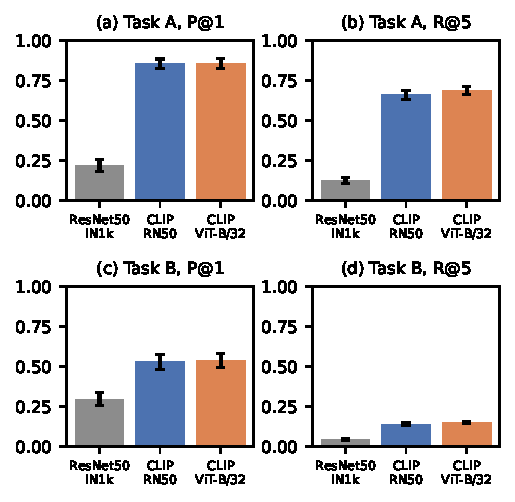
\includegraphics[width=\columnwidth]{figures/fig_vlm_comparison.pdf}
    \caption{ResNet50-IN1kとCLIPの指標の比較．誤差棒は画像単位のブートストラップ95\%信頼区間である．}
    \label{fig_vlm_comparison}
\end{figure}

表\ref{tab_vlm_comparison}と図\ref{fig_vlm_comparison}に結果を示す．
ResNet50-IN1kとCLIP系の間には，タスクA・タスクBの全指標において統計的に有意な差が認められた．
p値は最大でもタスクBのR@1における$ 2.2 \times 10^{-12} $であった．
ResNet50-IN1kはCOCOのクラス名の多くと一致するImageNetのクラスを持たないため，例えば``person''に対するスコアは常に0となる．
この結果は，カテゴリのアノテーションには固定のクラス集合に縛られないVLMが必要であることを示している．

一方，CLIP-RN50とCLIP-ViT-B/32の間では，P@1とR@1には有意な差が認められなかった（$ p \geq 0.53 $）．
P@5とR@5ではCLIP-ViT-B/32がわずかに高く，有意な差が認められた（タスクAのR@5で$ p = 6.3 \times 10^{-4} $，タスクBのP@5で$ p = 2.8 \times 10^{-3} $）．
両CLIPの差は，ResNet50-IN1kとの差と比べて1桁以上小さい．
この結果は，$ f $の性能差において「学習手法・語彙設計（クラス分類か，対照学習によるオープンボキャブラリ化か）」の要因が「モデル構造（CNNかViTか）」の要因よりも支配的であることを示唆している．

\subsection{物体領域検出モデルの選択}
本研究ではカテゴリに依存しない検出のみを行うDETRを物体領域の検出に採用する．
この選択が位置検出精度の観点からも妥当であることを確認するため，DETRと，オープンボキャブラリ物体検出モデルであるOWL-ViT（owlvit-base-patch32）\cite{ref_OWLViT}，Grounding DINO（grounding-dino-tiny）\cite{ref_GDINO}の3手法を比較した．
OWL-ViTとGrounding DINOには，COCOの80クラス名をテキストクエリとして与え，予測カテゴリを捨ててクラス間でNMS（IoU 0.5）を行うことで，クラス非依存のボックス集合とした．
検出スコアの閾値はOWL-ViTを0.1，Grounding DINOをbox 0.35・text 0.25とし，DETRは$ \theta \in \{0.5, 0.7, 0.9\} $を比較した．
評価には，500枚のうちGTインスタンスが2〜3件の画像をサンプリング順に走査し，GTインスタンスの合計が10件となる最初の4枚の組を用いた．
評価指標は，GTインスタンスに対しIntersection over Union（IoU）が0.5以上の提案が存在する割合（Recall@IoU0.5）と，GTインスタンスごとの提案との最良IoUの平均値（平均最良IoU）である．

\begin{table}[t]
    \centering
    \caption{物体領域検出モデルの比較（4画像，GTインスタンス10件）．RecallはRecall@IoU0.5である．}
    \label{tab_detectors}
    \footnotesize
    \setlength{\tabcolsep}{3pt}
    \begin{tabular}{lcccc}
        \toprule
        手法 & 閾値 & 平均提案数 & Recall & 平均最良IoU \\
        \midrule
        DETR           & 0.5  & 2.25 & {\bf 0.800} & 0.705 \\
        DETR           & 0.7  & 1.75 & 0.700 & 0.669 \\
        DETR           & 0.9  & 1.50 & 0.600 & 0.583 \\
        OWL-ViT        & 0.1  & 1.50 & 0.500 & 0.517 \\
        Grounding DINO & 0.35 & 1.50 & 0.500 & 0.546 \\
        YOLO11x & 0.25 & 2.25 & 0.700 & 0.719 \\
        YOLOv8x & 0.25 & 2.25 & 0.800 & {\bf 0.767} \\
        \bottomrule
    \end{tabular}
\end{table}

表\ref{tab_detectors}に結果を示す．
平均提案数をそろえた条件（DETRの$ \theta = 0.9 $）でも，DETRのRecall@IoU0.5と平均最良IoUはOWL-ViTおよびGrounding DINOと同等以上であった．
3手法ともRecallが1.0に達しない原因を調べたところ，画像面積の0.3\%しかない遠方の車と，画像のほぼ全体（面積比98\%）を占める食卓のGTが，全手法で検出されていなかった．
したがって，位置検出精度の観点からOWL-ViTやGrounding DINOを用いる利点は認められない．
一方，OWL-ViTとGrounding DINOは候補カテゴリ集合を検出処理の入力として必要とするため，カテゴリの粒度を変更するたびに検出処理そのものを再実行する必要がある．
DETRはカテゴリに依存しない検出を1回行えばよく，同一の検出結果を後段の処理全体で再利用できる．
本研究ではこの設計上の利点に基づき，DETRを採用する．
なお，4.8節で用いるYOLO11xとYOLOv8x（検出スコアの閾値0.25）を同じ4画像で評価したところ，Recall@IoU0.5はそれぞれ0.700，0.800，平均最良IoUは0.719，0.767であり，DETR（$ \theta = 0.5 $）と同程度であった．
ただし，4画像・10インスタンスによる比較であり，統計的な結論を得るには評価規模の拡大が必要である．

\subsection{カテゴリのアノテーションの精度}
提案するパイプライン全体としてのカテゴリアノテーション精度を評価した．
500枚に対しDETRを1回ずつ実行し，検出ボックスとGTボックスをハンガリアン法\cite{ref_Hungarian}によりIoU 0.5以上で1対1に対応付けた組を評価インスタンスとした．
候補語彙集合をCOCOの80クラスとし，各インスタンスのクロップに(\ref{eq_argmax})を適用して，推定単語がGTカテゴリと一致する割合（Top-1正解率）と，上位5語にGTカテゴリが含まれる割合（Top-5正解率）を計算した．
検出スコアの閾値$ \theta \in \{0.5, 0.7, 0.9, 0.97\} $と，3.3節で述べたクロップの前処理（center，pad）を変化させた．

\begin{table}[t]
    \centering
    \caption{パイプライン全体のカテゴリアノテーション精度．$ n $は評価インスタンス数である．}
    \label{tab_pipeline_accuracy}
    \small
    \setlength{\tabcolsep}{4pt}
    \begin{tabular}{ccccccc}
        \toprule
        \multirow{2}{*}{$ \theta $} & \multirow{2}{*}{前処理} & \multirow{2}{*}{$ n $} & \multicolumn{2}{c}{CLIP-ViT-B/32} & \multicolumn{2}{c}{CLIP-RN50} \\
        & & & Top-1 & Top-5 & Top-1 & Top-5 \\
        \midrule
        0.5  & center & 2343 & 0.481 & 0.778 & 0.367 & 0.649 \\
        0.7  & center & 2217 & 0.488 & 0.783 & 0.371 & 0.655 \\
        0.9  & center & 1892 & 0.506 & 0.804 & 0.389 & 0.681 \\
        0.97 & center & 1519 & 0.525 & 0.830 & 0.408 & 0.709 \\
        \midrule
        0.5  & pad    & 2343 & 0.560 & 0.855 & 0.460 & 0.740 \\
        0.7  & pad    & 2217 & 0.568 & 0.858 & 0.467 & 0.747 \\
        0.9  & pad    & 1892 & 0.587 & 0.874 & 0.484 & 0.776 \\
        0.97 & pad    & 1519 & {\bf 0.604} & {\bf 0.894} & 0.512 & 0.808 \\
        \bottomrule
    \end{tabular}
\end{table}

\begin{figure}[t]
    \centering
    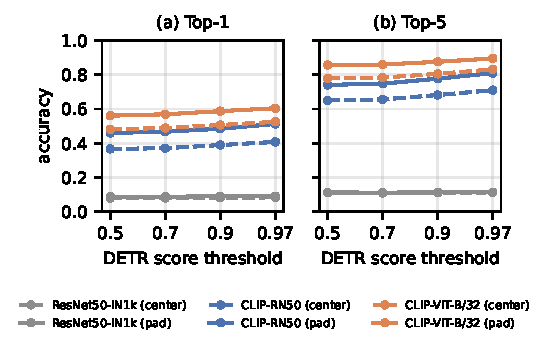
\includegraphics[width=\columnwidth]{figures/fig_pipeline_accuracy.pdf}
    \caption{DETRの検出スコアの閾値に対するカテゴリアノテーション精度．破線はcenter，実線はpadである．}
    \label{fig_pipeline_accuracy}
\end{figure}

表\ref{tab_pipeline_accuracy}と図\ref{fig_pipeline_accuracy}に結果を示す．
CLIP-ViT-B/32，$ \theta = 0.97 $，padの設定で，Top-1正解率0.604，Top-5正解率0.894が得られた．
CLIPの2モデルでは，すべての閾値においてpadはcenterよりTop-1正解率が0.08〜0.10高かった．
例えば$ \theta = 0.97 $のCLIP-ViT-B/32では，padによって正解に転じたインスタンスが217件，逆に不正解に転じたインスタンスが97件であった．
クラス別では，bottleの正解率が0.344から0.844へ，carの正解率が0.378から0.581へ向上した．
図\ref{fig_crop_preprocess}に例を示す．
縦長のボトルのクロップはcenterではラベル部分だけが残り``book''と推定されたが，padでは全体形状が保たれて``bottle''と推定された．
また，閾値を高くするほど正解率は単調に向上した．
これは，検出スコアの高い，すなわち明瞭に写った物体のみが評価対象として残るためと考えられる．
なお，同じパイプラインにResNet50-IN1kを用いた場合のTop-1正解率は全条件で0.09以下であり，4.2節の結論と整合する．

\begin{figure}[t]
    \centering
    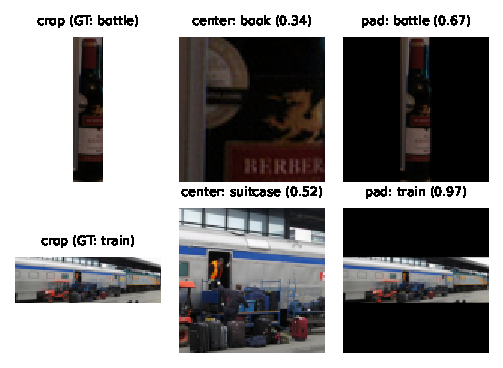
\includegraphics[width=\columnwidth]{figures/fig_crop_preprocess.pdf}
    \caption{クロップの前処理によるVLMへの入力の違い．左からクロップ，centerでVLMに入力される領域，padの入力であり，見出しは推定単語と確信度である．}
    \label{fig_crop_preprocess}
\end{figure}

一方，人物クラスの正解率は前処理によらず低く，$ \theta = 0.97 $でcenterが0.377，padが0.383であった．
人物は評価インスタンスの34\%を占め，主な誤りはperson → baseball bat（38件），skateboard（27件），tie（26件），tennis racket（24件）であった．
これは，人物が持っている物や身に着けている物に対してCLIPが強く反応するためであり，前処理では解消されない誤りである．

\subsection{WordNetによる粒度可変アノテーションにおける確信度の評価}
3.4節で述べたWordNet階層を用いた粒度可変アノテーションについて，各深さにおけるVLMの確信度を評価した．
COCOの80クラス（深さ0）についてはGTカテゴリとの正誤を判定できるが，それより細かい粒度についてはCOCOにGTが存在せず正誤を判定できない．
そこで，4.4節の最良の設定（CLIP-ViT-B/32，$ \theta = 0.97 $，pad）において深さ0の推定がGTカテゴリと一致した917件を対象に，深さを増すにつれて確信度がどのように変化するかを調べた．
最大深さは設けず，下位語集合が空になるまで細分化を繰り返した．

\begin{table}[b]
    \centering
    \caption{WordNet階層の深さごとの統計．単一は候補語彙が1語のみの段階の数，除外は単一の段階を除いた平均確信度である．}
    \label{tab_depth}
    \footnotesize
    \setlength{\tabcolsep}{3.5pt}
    \begin{tabular}{cccccc}
        \toprule
        深さ$ d $ & インスタンス数 & 平均候補数 & 平均確信度 & 単一 & 除外 \\
        \midrule
        0 & 917 & 80.0  & 0.642 & 0   & 0.642 \\
        1 & 784 & 108.8 & 0.442 & 80  & 0.378 \\
        2 & 328 & 6.2   & 0.715 & 110 & 0.571 \\
        3 & 54  & 14.5  & 0.577 & 10  & 0.481 \\
        4 & 18  & 5.7   & 0.755 & 9   & 0.511 \\
        5 & 4   & 10.8  & 0.406 & 0   & 0.406 \\
        \bottomrule
    \end{tabular}
\end{table}

\begin{figure}[t]
    \centering
    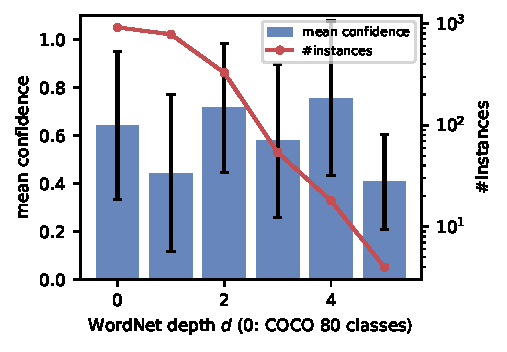
\includegraphics[width=\columnwidth]{figures/fig_depth_confidence.pdf}
    \caption{WordNet階層の深さごとの平均確信度（棒，左軸，誤差棒は標準偏差）とインスタンス数（折れ線，右軸，対数）．}
    \label{fig_depth_confidence}
\end{figure}

表\ref{tab_depth}と図\ref{fig_depth_confidence}に結果を示す．
深さ0から深さ1にかけて，平均確信度は0.642から0.442へ大きく低下した．
深さ1では，候補語彙数がCOCOの80クラスから平均108.8語へ増加し，かつ視覚的に類似した細かいカテゴリ間の識別が求められる．
特に\texttt{person.n.01}の直接の下位語は398語あり，深さ1の候補数の平均を押し上げている．
深さ2以降の平均確信度は0.715，0.577，0.755と変動しており，深さ1のように単調に低下する傾向は見られない．
しかし，(\ref{eq_clip})より候補語彙が1語のみの段階では確信度が必ず1となる．
このような段階は深さ1以降の全1188段階のうち209段階（約18\%）あり，特に深さ2では328段階中110段階を占めた．
これらを除いた平均確信度は，深さ1で0.378，深さ2で0.571，深さ3で0.481であり，深さ2以降の見かけの確信度の高さの一部は単一候補の分岐によるものである．
また，深さ3以降のインスタンス数は数件〜数十件と急減するため，これらの深さにおける確信度の変動を一般的な傾向として解釈することはできない．
深さ2以降のインスタンス数の急減は，大多数のCOCOカテゴリのWordNet下位語ツリーが浅いことを反映している．

\subsection{COCO以外の語を含む実画像へのアノテーション}
本手法の開語彙性がCOCOの80クラスという評価用データセットの語彙に限定されないことを確認するため，COCOに含まれない語を主要な被写体とする実画像に対するアノテーションを実施した．
第1段階の候補語彙集合として，COCOの80クラスに加え，penguin，helicopter，kangaroo，camel，lighthouse等，COCOに含まれない22語を手動で追加した計102語からなる語彙集合を用いた．
評価対象の画像には，Wikimedia Commonsで公開されている，ペンギン，ヘリコプター，ラクダ，カンガルー，灯台の写真6枚を用いた．
灯台については構図の異なる2枚を用いた．
DETRの閾値は$ \theta = 0.5 $，前処理はpadとした．

\begin{figure*}[t]
    \centering
    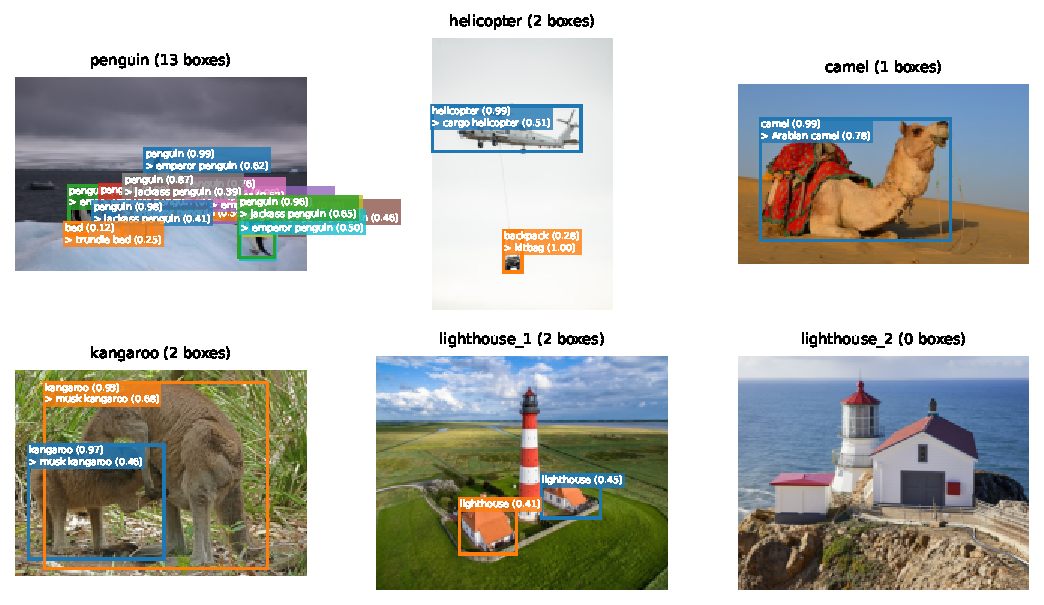
\includegraphics[width=0.95\textwidth]{figures/fig_open_vocab.pdf}
    \caption{COCO以外の語を含む実画像へのアノテーション結果．各ボックスに各段階の推定単語と確信度を示す．画像はWikimedia Commons（CC BY 2.0，CC0，CC BY-SA 3.0/4.0）より取得した．}
    \label{fig_open_vocab}
\end{figure*}

図\ref{fig_open_vocab}に結果を示す．
ペンギン，ヘリコプター，ラクダ，カンガルーの4枚については，DETRが物体領域を検出し，第1段階でいずれも正しい語（``penguin''，``helicopter''，``camel''，``kangaroo''）がアノテーションされた．
主要被写体の確信度は0.74〜0.99であった．
さらに下位語の段階では，ラクダの画像で``camel'' → ``Arabian camel''（確信度0.78）という妥当な細分化が得られた．
一方，アデリーペンギンの画像では，候補に``adelie''が含まれるにもかかわらず``emperor penguin''や``jackass penguin''が選ばれ，細分化は不正確であった．
灯台の画像については，2枚のいずれにおいても灯台の塔そのものは検出されなかった．
1枚目では塔の隣の家屋2棟が検出され，それらに``lighthouse''（確信度0.41，0.45）が付与された．
2枚目では検出スコア0.5以上のボックスが1件も出力されなかった．
これは，DETRがカテゴリに依存しない検出器として利用されている場合でも，その領域提案の性質はCOCOの学習データの分布から完全には独立ではなく，COCOのいずれのカテゴリとも視覚的に大きく異なる物体に対しては検出自体に失敗し得ることを示している．

また，ヘリコプターの画像では，機体の``helicopter''（確信度0.99）に加え，吊り下げられた車両の小領域が``backpack''（確信度0.28）→ ``kitbag''とアノテーションされた．
この領域は候補語彙中に適切な語が存在しないため，最も類似度の高い無関係な語が選択されたと考えられる．
開語彙アノテーションにおいて，候補語彙に正解語が含まれない領域への対処が今後の課題であることを示している．

\subsection{定性的結果}
図\ref{fig_coco_qualitative}に，COCOの画像に対する階層的アノテーションの結果を示す．
猫の領域は``cat'' → ``domestic cat''（確信度0.95）と妥当に細分化された．
一方，キリンの画像では6領域すべてが``giraffe''の下位語段階で``okapi''（キリン科の近縁種であるオカピ）に細分化された．
これは\texttt{giraffe.n.01}の下位語がokapiの1語のみであり，候補選択が実質的に機能していないためである．
同様に，象の画像では``Indian elephant''の唯一の下位語である``white elephant''（アルビノのインドゾウ）が，熊の画像では``American black bear''の唯一の下位語である``cinnamon bear''が，いずれも確信度1.00で選ばれた．
4.5節で定量的に示したとおり，このような単一候補の分岐は例外的なものではなく，okapi（28件），spindlelegs（24件），moped（18件）等，COCOの評価インスタンス全体にわたって再現している．

\begin{figure*}[t]
    \centering
    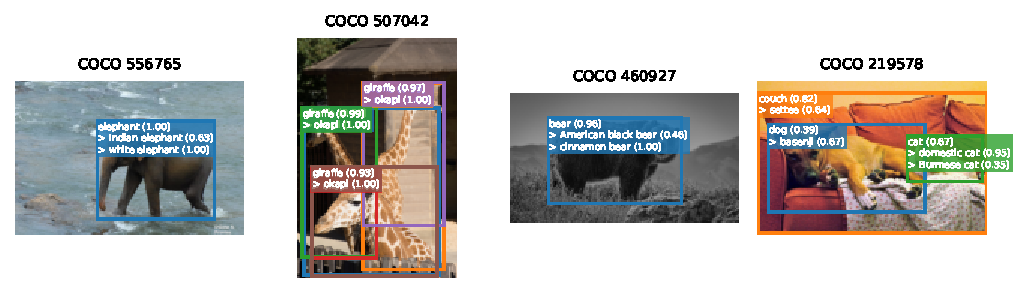
\includegraphics[width=0.95\textwidth]{figures/fig_coco_qualitative.pdf}
    \caption{WordNetによる粒度可変アノテーションの定性的結果．左から，象，キリン，熊，犬と猫とソファの画像である．}
    \label{fig_coco_qualitative}
\end{figure*}

\subsection{閉域物体検出モデルYOLOとの比較}
提案手法の第1段階は，COCOの80クラスを候補語彙とするため，COCOの80クラスで学習した閉域物体検出モデルと同じ語彙でアノテーションを行う．
そこで，YOLO自体の語彙であるCOCOの80クラスを用いて，提案手法とYOLOを比較した．
YOLOには，Ultralytics\cite{ref_Ultralytics}の学習済みモデルであるYOLO11n，YOLO11m，YOLO11x，YOLOv8xを用いた．
これらはCOCO train2017で学習されており，評価に用いるval2017は学習データに含まれない．
YOLOの検出スコアの閾値は既定値の0.25に加えて0.5と0.7を比較し，NMSのIoU閾値は既定値の0.7とした．
4.4節と同じ500枚に対し，YOLOの検出ボックスとGTボックスをハンガリアン法によりIoU 0.5以上で1対1に対応付け，YOLOが出力したクラスによるTop-1正解率と，80クラスのスコアの上位5件によるTop-5正解率を計算した．
また，対応付けられるインスタンスの数は手法や閾値によって異なるため，GTインスタンス全体のうち正しいカテゴリでアノテーションされた割合を正命名率

\begin{equation}
    r = \frac{N_{\mathrm{correct}}}{N_{\mathrm{GT}}}
    \label{eq_annotation_recall}
\end{equation}

\noindent
として計算した．
ここで，$ N_{\mathrm{correct}} $はTop-1の推定がGTカテゴリと一致したインスタンス数，$ N_{\mathrm{GT}} $はGTインスタンスの総数（3206件）である．

\begin{table}[t]
    \centering
    \caption{YOLOと提案手法のカテゴリアノテーション精度（COCOの80クラス）．閾値は提案手法では$ \theta $，YOLOでは検出スコアの閾値，$ r $は正命名率である．}
    \label{tab_yolo_comparison}
    \footnotesize
    \setlength{\tabcolsep}{3pt}
    \begin{tabular}{lccccc}
        \toprule
        手法 & 閾値 & $ n $ & Top-1 & Top-5 & $ r $ \\
        \midrule
        提案手法          & 0.5  & 2343 & 0.560 & 0.855 & 0.410 \\
        提案手法          & 0.97 & 1519 & 0.604 & 0.894 & 0.286 \\
        \midrule
        YOLO11n          & 0.25 & 1717 & 0.957 & 0.996 & 0.513 \\
        YOLO11m          & 0.25 & 2115 & 0.976 & 0.998 & 0.644 \\
        YOLO11x          & 0.25 & 2210 & 0.981 & 0.999 & {\bf 0.676} \\
        YOLO11x          & 0.7  & 1474 & {\bf 0.993} & 0.997 & 0.456 \\
        YOLOv8x          & 0.25 & 2220 & 0.971 & 0.999 & 0.672 \\
        \midrule
        YOLO11x + CLIP   & 0.25 & 2210 & 0.565 & 0.860 & 0.390 \\
        YOLO11x + CLIP   & 0.7  & 1474 & 0.604 & 0.907 & 0.278 \\
        \bottomrule
    \end{tabular}
\end{table}

\begin{figure}[t]
    \centering
    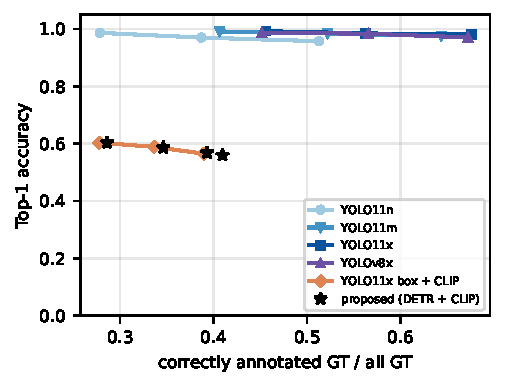
\includegraphics[width=\columnwidth]{figures/fig_yolo_comparison.pdf}
    \caption{正命名率（横軸）と，対応付けられたインスタンスにおけるTop-1正解率（縦軸）の関係．YOLOは検出スコアの閾値0.25，0.5，0.7，提案手法は$ \theta = 0.5, 0.7, 0.9, 0.97 $の結果である．}
    \label{fig_yolo_comparison}
\end{figure}

表\ref{tab_yolo_comparison}と図\ref{fig_yolo_comparison}に結果を示す．
COCOの80クラスの範囲内では，YOLOのTop-1正解率は0.957〜0.993であり，提案手法の0.560〜0.604を大きく上回った．
正命名率もYOLO11xの0.676に対し提案手法は0.410であり，YOLOの方が高い．
両手法が検出した共通のGTインスタンスに限定して比較しても，YOLO11x（閾値0.25）と提案手法（$ \theta = 0.97 $）に共通する1480件において，Top-1正解率はYOLO11xが0.989，提案手法が0.609であった．
YOLO11xのみが正解した件数は570件，提案手法のみが正解した件数は8件であり，McNemar検定で有意な差が認められた（$ p < 10^{-150} $）．
人物クラスに限ると，YOLO11xの正解率は0.998であるのに対し，提案手法は0.379であり，4.4節で述べた人物クロップの誤りが差の大きな部分を占める．
ただし，人物以外のクラスでも，YOLO11xが0.984，提案手法が0.732と差があった．

この差が検出器と分類器のいずれに起因するかを切り分けるため，YOLO11xの検出ボックスのクロップをpadの前処理でCLIP-ViT-B/32に入力して分類する組合せ（YOLO11x + CLIP）を評価した．
その結果，Top-1正解率は0.565〜0.604となり，インスタンス数が同程度の提案手法とほぼ一致した．
例えば，YOLO11x + CLIPの閾値0.7（1474件）と提案手法の$ \theta = 0.97 $（1519件）は，いずれもTop-1正解率が0.604であった．
したがって，COCOの80クラスの範囲内でのYOLOとの差は検出器ではなく，COCOの80クラスで教師あり学習されたYOLOの分類と，ゼロショットのCLIPによる分類との精度の差に起因する．

\begin{figure*}[t]
    \centering
    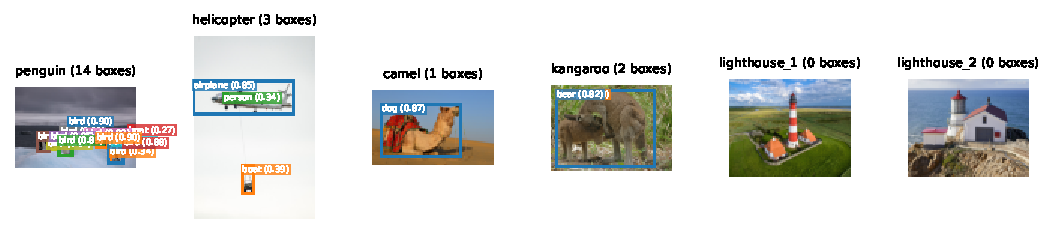
\includegraphics[width=0.95\textwidth]{figures/fig_yolo_open_vocab.pdf}
    \caption{COCO以外の語を含む実画像に対するYOLO11x（検出スコアの閾値0.25）の検出結果．各ボックスにYOLOが出力したクラスと検出スコアを示す．}
    \label{fig_yolo_open_vocab}
\end{figure*}

一方，図\ref{fig_yolo_open_vocab}に示すとおり，4.6節のCOCO以外の語を含む実画像に対しては，YOLO11xはペンギンを``bird''，ラクダを``dog''，カンガルーを``bear''と``sheep''，ヘリコプターを``airplane''とアノテーションした．
YOLOは学習した80クラスの語しか出力できないため，これらの物体を正しく命名することは原理的にできない．
同じ画像に対し，提案手法は``penguin''，``camel''，``kangaroo''，``helicopter''を正しくアノテーションしている（図\ref{fig_open_vocab}）．
また，灯台の画像2枚では，YOLO11xも検出スコア0.25以上のボックスを1件も出力しなかった．

\subsection{YOLOとVLMを組み合わせた粒度可変アノテーション}
4.8節の結果から，COCOの80クラスの範囲内ではYOLOの分類が提案手法のゼロショット分類を大きく上回る．
一方，3.4節の粒度可変アノテーションは深さ0の推定結果から下位語をたどるため，深さ0で誤った単語を選ぶと，以降の段階でも誤った分岐をたどる．
そこで，深さ0のカテゴリをYOLOの予測とし，深さ1以降の細分化のみをVLMとWordNetで行う構成（以下，ハイブリッド構成）を評価した．
YOLOが出力した領域$ k $のボックスを$ {\mathbf b}_k $，クラスを$ y_k \in {\mathbb V}^{(0)} $とし，(\ref{eq_crop})のクロップ$ {\mathbf X}_k $に対して(\ref{eq_hyponym})により深さ1以降の単語を推定する．
ただし，YOLOは80クラス以外の語を出力できないため，4.6節のCOCO外の22語の集合を$ {\mathbb V}_E $とし，COCO外の物体に対してはVLMの推定に切り替える規則

\begin{equation}
    \hat{v}_k^{(0)} =
    \begin{cases}
        u_k & (u_k \in {\mathbb V}_E \ \text{かつ}\ f({\mathbf X}_k; {\mathbb V}^{(0)} \cup {\mathbb V}_E)_{u_k} \geq \gamma) \\
        y_k & (\text{それ以外})
    \end{cases}
    \label{eq_hybrid_switch}
\end{equation}

\noindent
を併せて評価した．
ここで，$ u_k $は102語の候補語彙$ {\mathbb V}^{(0)} \cup {\mathbb V}_E $を用いて(\ref{eq_argmax})により推定した単語，$ \gamma $は切替に必要な確信度の下限である．
YOLOにはYOLO11x（検出スコアの閾値0.25，0.5，0.7），$ f $にはCLIP-ViT-B/32を用い，クロップの前処理はpadとした．
切替については，切替を行わない構成，$ \gamma = 0 $，$ \gamma = 0.5 $の3通りを比較した．
なお，$ \gamma = 0.5 $は$ \gamma = 0 $の結果を確認した後に追加した設定である\add{ため，4.10節で別の500枚を用いて検証する}．
評価には4.8節と同じ対応付けを用い，深さ0の推定がGTカテゴリと一致したインスタンス数を，深さ1以降の階層的アノテーションの対象となるインスタンス数$ N_h $とした．
深さ1以降はCOCOに正解が存在しないため，4.5節と同様に正誤は評価せず，両手法の深さ0が正解となった共通のGTインスタンスにおける深さ1の推定単語の一致率を求めた．

\begin{table}[t]
    \centering
    \caption{ハイブリッド構成と提案手法の比較（COCOの80クラス，500枚）．閾値は提案手法では$ \theta $，ハイブリッド構成ではYOLO11xの検出スコアの閾値である．一致率は提案手法（$ \theta = 0.97 $）と共通のインスタンスにおける深さ1の推定単語の一致率である．}
    \label{tab_hybrid}
    \footnotesize
    \setlength{\tabcolsep}{2.5pt}
    \begin{tabular}{lcccccc}
        \toprule
        手法 & 閾値 & $ n $ & Top-1 & $ r $ & $ N_h $ & 一致率 \\
        \midrule
        提案手法                     & 0.5  & 2343 & 0.560 & 0.410 & 1313 & -- \\
        提案手法                     & 0.97 & 1519 & 0.604 & 0.286 & 917  & -- \\
        \midrule
        ハイブリッド（切替なし）     & 0.25 & 2210 & 0.981 & 0.676 & 2167 & 0.775 \\
        ハイブリッド（切替なし）     & 0.5  & 1832 & 0.985 & 0.563 & 1804 & 0.776 \\
        ハイブリッド（切替なし）     & 0.7  & 1474 & 0.993 & 0.456 & 1463 & 0.796 \\
        ハイブリッド（$ \gamma = 0 $） & 0.25 & 2210 & 0.959 & 0.661 & 2120 & 0.780 \\
        ハイブリッド（$ \gamma = 0 $） & 0.7  & 1474 & 0.974 & 0.448 & 1436 & 0.799 \\
        \bottomrule
    \end{tabular}
\end{table}

\begin{figure*}[t]
    \centering
    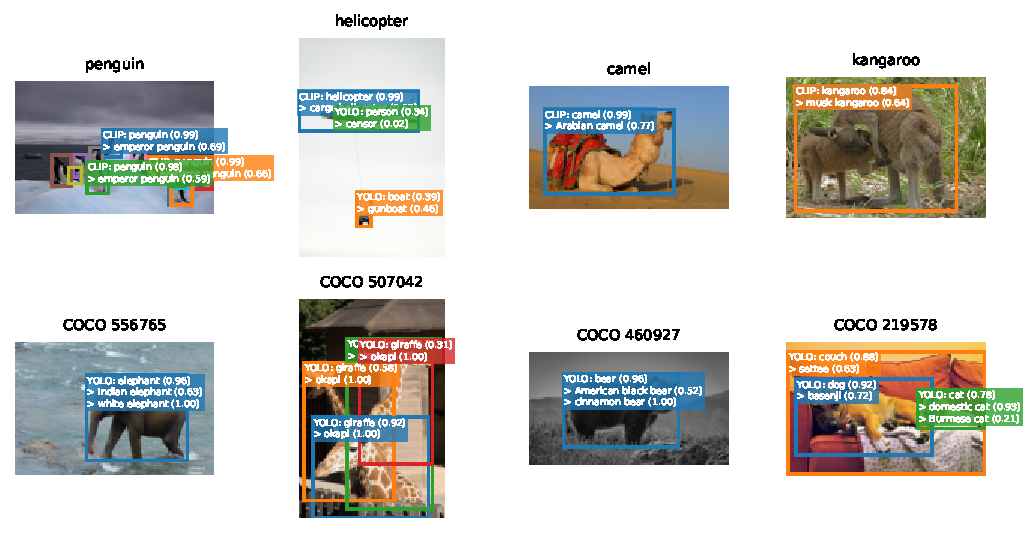
\includegraphics[width=0.95\textwidth]{figures/fig_hybrid_qualitative.pdf}
    \caption{ハイブリッド構成（YOLO11xの検出スコアの閾値0.25，$ \gamma = 0.5 $）による粒度可変アノテーションの定性的結果．上段はCOCO以外の語を含む実画像，下段は図\ref{fig_coco_qualitative}と同じCOCOの画像である．深さ0の単語の前に，その決定に用いたモデルを``YOLO:''，``CLIP:''で示す．ペンギンの画像では検出スコアの上位3件のみ単語を表示している．}
    \label{fig_hybrid_qualitative}
\end{figure*}

表\ref{tab_hybrid}に結果を示す．
切替を行わない構成では，深さ0のTop-1正解率はYOLO11xと同じ0.981〜0.993となり，階層的アノテーションの対象となるインスタンス数$ N_h $は，閾値0.25で2167件であった．
\add{ただし，提案手法の$ \theta $とYOLO11xの閾値は検出スコアの定義が異なり，数値を直接対応させることはできない．そこで，評価インスタンス数$ n $が近い組で比較すると，$ N_h $は提案手法の$ \theta = 0.5 $（$ n = 2343 $）の1313件に対しYOLO11xの閾値0.25（$ n = 2210 $）で2167件と1.65倍，$ \theta = 0.97 $（$ n = 1519 $）の917件に対し閾値0.7（$ n = 1474 $）で1463件と1.60倍であった．}
したがって，ハイブリッド構成により，深さ0の誤りによって誤った分岐をたどるインスタンスを減らしつつ，より多くのGTインスタンスに粒度可変のアノテーションを付与できる．

深さ1の平均確信度は，ハイブリッド構成（閾値0.25）で0.366であり，提案手法（$ \theta = 0.97 $）の0.442より低かった．
これは，提案手法では正解率の低い人物クラスがハイブリッド構成では正しく推定され，候補語彙数の多い\texttt{person.n.01}の下位語（平均398語）をたどるインスタンスが増えたためである．
人物クラスは対象インスタンスの32.9\%を占め，深さ1の平均確信度は0.080であった．
人物クラス以外に限ると，深さ1の平均確信度はハイブリッド構成で0.537，提案手法で0.572であり，その差は小さい．
また，両手法に共通する761件における深さ1の推定単語の一致率は0.775であった．
両手法は同じCLIPで細分化を行うため，約2割の不一致はDETRとYOLOのボックスの違いに起因する．
すなわち，細かい粒度の推定は入力するクロップのわずかな違いによって変化しうる．

COCO外の語への切替を$ \gamma = 0 $で行うと，閾値0.25において47件の領域でCOCO外の語に切り替わり，そのすべてがYOLOでは正解していたインスタンスであった．
例えば，羊がcamelに（8件），人物がdolphin，monkey，penguin等に切り替わっており，深さ0のTop-1正解率は0.981から0.959に低下した．
一方，$ \gamma = 0.5 $では，\add{切替は閾値0.25で2件，0.5で2件，0.7で1件に減少し，深さ0のTop-1正解率は閾値0.25で0.980であった．ただし，切り替わった領域は羊（camel，確信度0.629）と鳥（eagle，確信度0.546）であり，いずれもYOLOでは正解していた．}
図\ref{fig_hybrid_qualitative}に，$ \gamma = 0.5 $のハイブリッド構成による定性的結果を示す．
YOLOがbird，airplane，dog，bearおよびsheepと出力したペンギン，ヘリコプター，ラクダ，カンガルーの領域は，CLIPの確信度0.78〜0.99でpenguin，helicopter，camel，kangarooに切り替わり，さらにemperor penguin，cargo helicopter，Arabian camel，musk kangarooへと細分化された．
また，COCOの犬と猫とソファの画像では，提案手法でcatやcouchと競合して確信度0.389であったdogが，YOLOにより検出スコア0.92で推定され，basenjiへと細分化された．
一方，giraffe → okapiのような下位語が1語しかない分岐は，深さ0の推定を変えても解消されない．
また，灯台の画像ではYOLO11xも領域を検出しないため，ハイブリッド構成でもアノテーションは得られない．

\begingroup
\color{red}
\subsection{別の画像による検証と深さ0の誤りの伝播}
4.4節から4.9節の評価では，検出スコアの閾値$ \theta $と$ \gamma $を，結果を報告する500枚と同じ画像で選んでいる．
また，深さ1以降の評価は深さ0が正解のインスタンスに限られ，深さ0の誤りが下位語へ伝播する影響は含まれていない．
そこで，COCO 2017 Validationの5000枚を，これまでの500枚（以下，検証用）と，それ以外の4500枚をseed 42で2等分した後半からサンプリングした500枚（以下，テスト用，GTインスタンス3748件）に分け，提案手法とハイブリッド構成をテスト用の500枚で再評価した．
さらに，深さ0の正誤によらず，全インスタンスについて下位語の集合が空になるまで(\ref{eq_hyponym})を適用した．
検出はDETRを$ \theta = 0.5 $，YOLO11xを閾値0.25で1回ずつ実行し，より高い閾値の結果は検出スコアによる絞り込みで得た．
検証用の500枚では，$ n $，Top-1正解率および$ N_h $がいずれも4.4節，4.8節，4.9節の値と一致した．

\begin{table}[t]
    \centering
    \caption{評価インスタンス数$ n $が近い組における提案手法とハイブリッド構成の比較．一致率は同じ組の両手法の深さ0が正解となった共通のGTインスタンスにおける深さ1の推定単語の一致率，誤りは深さ0が不正解のまま下位語へ展開されたインスタンスの割合である．}
    \label{tab_eval_pairs}
    \footnotesize
    \setlength{\tabcolsep}{2.5pt}
    \begin{tabular}{llcccccc}
        \toprule
        分割 & 手法 & 閾値 & $ n $ & Top-1 & $ N_h $ & 誤り & 一致率 \\
        \midrule
        \multirow{4}{*}{検証用} & 提案手法     & 0.5  & 2343 & 0.560 & 1313 & 0.440 & \multirow{2}{*}{0.751} \\
                                & ハイブリッド & 0.25 & 2210 & 0.981 & 2167 & 0.019 & \\
                                & 提案手法     & 0.97 & 1519 & 0.604 & 917  & 0.396 & \multirow{2}{*}{0.796} \\
                                & ハイブリッド & 0.7  & 1474 & 0.993 & 1463 & 0.007 & \\
        \midrule
        \multirow{4}{*}{テスト用} & 提案手法     & 0.5  & 2736 & 0.552 & 1509 & 0.448 & \multirow{2}{*}{0.704} \\
                                  & ハイブリッド & 0.25 & 2572 & 0.969 & 2492 & 0.031 & \\
                                  & 提案手法     & 0.97 & 1669 & 0.625 & 1043 & 0.375 & \multirow{2}{*}{0.750} \\
                                  & ハイブリッド & 0.7  & 1584 & 0.982 & 1556 & 0.018 & \\
        \bottomrule
    \end{tabular}
\end{table}

表\ref{tab_eval_pairs}に結果を示す．
テスト用の500枚においても，ハイブリッド構成の$ N_h $は提案手法の1.65倍（閾値0.25と$ \theta = 0.5 $）および1.49倍（閾値0.7と$ \theta = 0.97 $）であり，4.9節の結論は別の画像でも成り立った．
一方，深さ1の推定単語の一致率はテスト用で0.704〜0.750であり，検出器が異なると約3割の物体で細分化の結果が異なった．

深さ0が不正解のまま下位語へ展開されたインスタンスは，テスト用の500枚において提案手法（$ \theta = 0.5 $）で2736件中1227件（44.8\%），ハイブリッド構成（閾値0.25）で2572件中80件（3.1\%）であった．
誤った枝における最も深い段階の平均確信度は，提案手法で0.473，ハイブリッド構成で0.637であり，ハイブリッド構成では正しい枝の0.547をむしろ上回った．
正しい枝と誤った枝を確信度によって区別できるかをArea Under the ROC Curve（AUROC）で評価すると，最も深い段階の確信度では提案手法で0.611，ハイブリッド構成で0.418，全段階の確信度の積では0.508，0.430であり，いずれもほぼ区別できなかった．
これに対し，深さ0の確信度では0.725，0.715であった．
すなわち，誤った語の下位語のみを候補とする深い段階の確信度は誤りの検出に役立たず，誤りの手がかりは深さ0の確信度に限られる．

最後に，テスト用の500枚で$ \gamma $による切替を確認した．
閾値0.25において，$ \gamma = 0 $では50件，$ \gamma = 0.5 $では8件の領域がCOCO外の語に切り替わり，深さ0のTop-1正解率はそれぞれ0.950，0.966であった．
ただし，$ \gamma = 0.5 $の8件のうち6件はbirdのGTに対するflamingo（4件），parrot，penguinであり，WordNetにおいてGTカテゴリの下位語である．
GTカテゴリの下位語でない切替は，$ \gamma = 0 $の41件に対し$ \gamma = 0.5 $では2件（bearに対するpanda，teddy bearに対するrabbit）であった．
したがって，検証用の500枚で選んだ$ \gamma = 0.5 $は，別の画像においても誤った切替の大部分を防いでいる．

\subsection{LVISを用いた深さ1以降の評価と累積確信度による細分化の停止}
深さ1以降の推定の正誤を評価するため，WordNetのSynsetが各カテゴリに付与されたLVIS v1\cite{ref_LVIS}のValidationのアノテーションを用いた．
LVISのアノテーションはCOCO 2017の画像に対して付与されており，本稿で用いたval2017の5000枚のうち4809枚にアノテーションが存在する．
COCOのGTに対応付けられた検出ボックスについて，IoUが0.5以上で，そのSynsetがGTカテゴリのSynsetの真の下位語であるLVISのアノテーションを細かい粒度の正解とした．
例えば，COCOのbirdに対するpigeon，bottleに対するwine bottleである．
画像の分割は，検証用の500枚と前述の4500枚の前半を検証用（2604枚），後半をテスト用（2148枚，前述のテスト用の500枚を含む）とし，テスト用の評価インスタンスは提案手法（$ \theta = 0.5 $）で489件，ハイブリッド構成（閾値0.25）で481件であった．

評価には，階層的分類で用いられる階層的適合率$ hP $，階層的再現率$ hR $およびその調和平均$ hF $\cite{ref_hF}を用いた．
インスタンス$ k $について，出力した各段階のSynsetの集合を$ {\mathbb P}_k $，GTカテゴリのSynsetからLVISのSynsetまでの経路上のSynsetの集合を$ {\mathbb G}_k $とし，

\begin{equation}
    hP = \frac{\sum_k |{\mathbb P}_k \cap {\mathbb G}_k|}{\sum_k |{\mathbb P}_k|}, \quad
    hR = \frac{\sum_k |{\mathbb P}_k \cap {\mathbb G}_k|}{\sum_k |{\mathbb G}_k|}
    \label{eq_hierarchical_pr}
\end{equation}

\noindent
とした．
ここで，LVISのSynsetより細かいSynsetは正誤を判定できないため$ {\mathbb P}_k $から除き，棄却したインスタンスでは$ {\mathbb P}_k $を空集合とした．

また，深さ0の誤りの伝播と深い段階の誤りを抑えるため，各段階の確信度の積である累積確信度

\begin{equation}
    c_k^{(d)} = \prod_{j=0}^{d} f({\mathbf X}_k; {\mathbb V}_k^{(j)})_{\hat{v}_k^{(j)}}
    \label{eq_cumulative_conf}
\end{equation}

\noindent
が閾値$ \tau $以上である最も深い段階までを出力し，$ c_k^{(0)} < \tau $の場合はアノテーションを棄却する停止規則を評価した．
ハイブリッド構成の深さ0では，$ f $の代わりにYOLO11xの検出スコアを用いた．
$ \tau $は検証用の分割で$ hF $が最大となる値を$ \{0, 0.001, \ldots, 0.9\} $の13通りから選び，テスト用の分割で評価した．
比較として，深さの上限で細分化を止める規則も評価した．
表\ref{tab_lvis_stopping}の「深さ1」は，深さ1で細分化を止める規則である．

\begin{table}[t]
    \centering
    \caption{LVISのテスト用分割における深さ1以降の評価．被覆率は棄却されなかったインスタンスの割合，Top-1は棄却されなかったインスタンスにおける深さ0のTop-1正解率，到達率はLVISのSynsetまで出力した割合である．$ \tau $は検証用の分割で選んだ値である．}
    \label{tab_lvis_stopping}
    \footnotesize
    \setlength{\tabcolsep}{2.0pt}
    \begin{tabular}{llcccccc}
        \toprule
        手法 & 停止規則 & 被覆率 & Top-1 & $ hP $ & $ hR $ & $ hF $ & 到達率 \\
        \midrule
        \multirow{3}{*}{\shortstack{提案手法\\$ \theta = 0.5 $}} & なし           & 1.000 & 0.646 & 0.425 & 0.430 & 0.428 & 0.272 \\
                                                                & 深さ1      & 1.000 & 0.646 & 0.490 & 0.417 & 0.451 & 0.256 \\
                                                                & $ \tau = 0.2 $ & 0.775 & 0.792 & 0.611 & 0.372 & 0.462 & 0.192 \\
        \midrule
        \multirow{3}{*}{\shortstack{ハイブリッド\\閾値0.25}} & なし           & 1.000 & 0.971 & 0.594 & 0.631 & 0.612 & 0.372 \\
                                                                & 深さ1      & 1.000 & 0.971 & 0.683 & 0.617 & 0.648 & 0.353 \\
                                                                & $ \tau = 0.3 $ & 0.975 & 0.970 & 0.801 & 0.543 & 0.647 & 0.237 \\
        \bottomrule
    \end{tabular}
\end{table}

\begin{figure}[t]
    \centering
    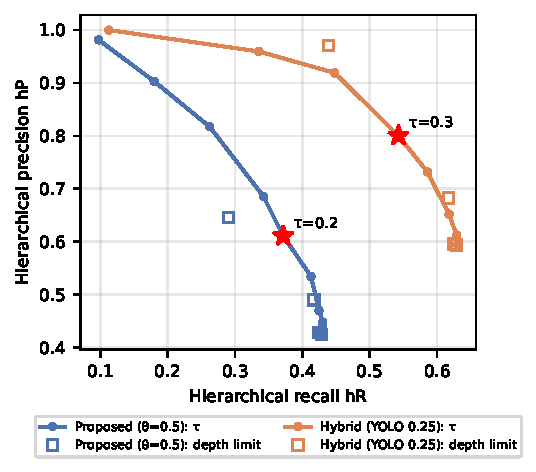
\includegraphics[width=0.85\columnwidth]{figures/fig_stopping.pdf}
    \caption{LVISのテスト用分割における階層的再現率$ hR $（横軸）と階層的適合率$ hP $（縦軸）の関係．実線は$ \tau $を変化させた累積確信度による停止規則，四角は深さの上限（0〜3）による停止規則，星印は検証用の分割で選んだ$ \tau $である．}
    \label{fig_stopping}
\end{figure}

表\ref{tab_lvis_stopping}と図\ref{fig_stopping}に結果を示す．
深さ0が正解のインスタンスにおける深さ1の推定単語がLVISの経路上にある割合は，提案手法で0.440，ハイブリッド構成で0.407であった．
すなわち，深さ0が正しくても，最初の細分化の段階で正しい下位語を選べたのは半数未満であり，4.5節で観測した確信度の低下は実際の誤りを伴っていた．
停止規則を用いない場合，$ hF $は提案手法で0.428，ハイブリッド構成で0.612であり，深さ0の精度の差がそのまま細かい粒度の精度の差となった．

累積確信度による停止規則では，検証用の分割で$ \tau = 0.2 $（提案手法）と$ \tau = 0.3 $（ハイブリッド構成）が選ばれ，テスト用の分割で$ hP $はそれぞれ0.425から0.611，0.594から0.801へ向上し，$ hF $も0.428から0.462，0.612から0.647へ向上した．
提案手法では，深さ0の確信度が$ \tau $未満である全インスタンスの22.5\%が棄却され，棄却されなかったインスタンスにおける深さ0のTop-1正解率が0.646から0.792へ向上した．
COCOのテスト用の500枚においても，同じ$ \tau = 0.2 $により，誤った枝の出力は1227件から703件へ減少し，正しい枝の出力は1509件から1242件となった．
一方，深さ1で細分化を止める単純な規則でも$ hF $は0.451，0.648であり，累積確信度による規則との差は小さかった．
これは，前節で示したように深さ1以降の確信度が正誤の手がかりにならず，停止規則の効果の多くが深さ0の確信度による棄却と，深い段階の出力の削減によって得られているためである．
\endgroup

\section{考察}
\subsection{従来手法との差別化点}
本研究の差別化点は，以下の3点に整理できる．

第一に，YOLO\cite{ref_YOLO}やDETR\cite{ref_DETR}のような閉域的な物体検出モデルに対しては，学習時に定めた固定のクラス集合を超えたカテゴリを予測できないという制約を解消している．
本手法では，DETRの予測カテゴリを用いず，バウンディングボックス出力のみを物体領域の検出に用いることで，検出済みの領域に対し後段のVLMが任意の候補語彙でカテゴリをアノテーションできるようにしている．
4.6節で確認したとおり，この設計により，COCOの80クラスに含まれない語（penguin，helicopter，kangaroo，camel）についても，追加学習なしにアノテーションが可能である．
\add{ただし，4.8節で示したとおり，COCOの80クラスの範囲内では，そのクラスで教師あり学習したYOLOの方がカテゴリのアノテーション精度は大幅に高い．本手法の利点は学習時の語彙を超えた語や粒度の異なる語でアノテーションできる点にあり，閉域の語彙で十分な用途ではYOLOのような閉域モデルが適している．}

第二に，OWL-ViT\cite{ref_OWLViT}やGrounding DINO\cite{ref_GDINO}のようなオープンボキャブラリ物体検出モデルに対しては，候補カテゴリ集合を変更するたびに検出処理全体を再実行する必要があるという制約を解消している．
4.3節で確認したとおり，位置検出精度はDETRとこれらのモデルの間で大きな差がないため，本手法は同等の位置検出精度を維持しつつ，物体領域の検出を1回のみに抑え，後段のカテゴリのアノテーションのみを候補語彙集合の変更に応じて繰り返す設計を実現している．

第三に，ImageNetのクラス階層を利用する従来の階層的画像分類の多くは，あらかじめ定めた固定の階層構造に対して学習を行うものであり，推論時に階層の深さや分岐を動的に選択することは想定していない．
本手法は，WordNetの上位語・下位語関係を推論時にたどることで，学習を一切行わずに粒度可変のアノテーションを実現している点で異なる．

\subsection{クロップの前処理と検出スコアの閾値の影響}
4.4節の結果は，同一のDETRとVLMを用いても，クロップの前処理と検出スコアの閾値によってTop-1正解率が0.481から0.604まで変化することを示している．
特に前処理の影響は，padでもcenterでも物体の外側の画像内容は含まないにもかかわらず，VLMの標準前処理である中央切り出しによって細長い物体の一部が失われることに起因する．
高さが幅の2倍以上のクロップでは，$ \theta = 0.9 $においてTop-1正解率がcenterの0.441からpadの0.545へ向上した．
クロップを入力とするVLMのゼロショット分類では，前処理を明示することが精度の比較に不可欠である．
一方，人物クラスでは前処理によらず正解率が0.38程度にとどまった．
人物のクロップには，人物とともにバット，ネクタイ，ラケット等の物体が含まれることが多く，``a photo of a person''よりもそれらの物体のプロンプトとの類似度が高くなる．
これは，候補語彙の中で包含関係にある物体同士をどのように扱うかという，クロップに基づくアノテーションに固有の課題である．

\subsection{WordNet階層をそのまま用いることの限界}
4.5節，4.7節の結果は，WordNetの生の階層構造をそのまま候補語彙として用いることに起因する2種類の限界を示している．

第一に，深さ0から深さ1への確信度の大幅な低下（0.642から0.442）に見られるように，候補語彙数の増加および視覚的に類似した細かいカテゴリ間の識別困難性により，最初の細分化の段階でアノテーションの信頼性が低下する．
さらに，\texttt{person.n.01}の下位語には``suspect''（20件），``thin person''（24件），``visually impaired person''（9件）等，外見だけからは判断できない社会的・属性的な語が多く含まれ，これらが実際に選択されていた．

第二に，giraffe → okapiのように，WordNetの階層構造には，視覚的なカテゴリ分類の候補語彙として不適切な分岐が含まれている．
特に下位語が1語しかない分岐では，(\ref{eq_clip})のソフトマックスにより確信度が画像によらず1となり，候補選択が実質的に機能しない．
このような段階は細分化の段階全体の約18\%を占め，深さ2以降の平均確信度を見かけ上押し上げていた．
単一候補の段階を除くと，深さ1から深さ3の平均確信度は0.378，0.571，0.481であり，深さ0と比べて一貫して低い．
これらの限界は，WordNetの階層構造が視覚的な類似性ではなく言語学的な意味関係に基づいて構築されていることに起因すると考えられる．

\subsection{物体領域の検出のCOCO学習分布への依存}
4.6節の灯台の事例は，カテゴリに依存しない検出器として利用する場合であっても，DETRの物体領域の検出そのものがCOCOの学習データの分布から完全には独立ではないことを示している．
すなわち，本手法における「物体領域の検出とカテゴリのアノテーションの分離」は，カテゴリの予測に関する制約を解消するものであるが，物体領域の候補生成そのものに関する制約は解消しない．
学習データに存在する物体の形状・構図との類似性への依存は残る．
また，ヘリコプターの吊り荷が``backpack''として誤ってアノテーションされた事例は，候補語彙集合に正解語が存在しない領域に対して，VLMが候補語彙中で最も類似度の高い無関係な語を選択してしまう問題を示している．

\subsection{今後の課題}
今後の課題として，第一に，WordNet階層のフィルタリングによる粒度可変アノテーションの実用性向上が挙げられる．
具体的には，下位語が1語しかない分岐の打ち切りや，絶滅種・希少種・外見から判断できない語の除外である．
第二に，物体領域の検出モデルの比較を本稿の4画像から500枚規模へ拡大し，統計的な比較を行うことが挙げられる．
第三に，物体領域の検出における学習分布への依存を緩和するため，Segment Anything Model（SAM）等の汎用的なセグメンテーションモデルとDETRを組み合わせるなど，物体領域の検出モデル自体の改善が挙げられる．
第四に，候補語彙に正解語が存在しない領域を棄却する仕組みとして，確信度に対する閾値処理の高度化や，候補語彙に「その他」に相当する語を加える方法の導入が挙げられる．
第五に，人物クロップにおける持ち物・装着物への誤反応を抑えるため，プロンプトの設計や，検出済みの他の領域との包含関係を考慮したアノテーションが挙げられる．
\add{第六に，4.8節の結果を踏まえ，COCOの80クラスで高精度なYOLOの予測を深さ0のアノテーションとして用い，深さ1以降の細分化と80クラスに含まれない語のアノテーションのみをVLMで行う組合せが挙げられる．}

\section{おわりに}
本稿では，画像中の物体らしい領域を検出するタスクと，その領域に対応するカテゴリをアノテーションするタスクを明確に分離する物体アノテーション手法を提案した．
物体領域の検出にはカテゴリに依存しない高精度なバウンディングボックスを1回の推論で出力するDETRを用い，カテゴリのアノテーションには検出済みの領域のクロップに対するVLMのゼロショット分類を用いた．
この分離により，一度検出した物体領域に対し，候補語彙集合を変更するだけで異なる粒度・異なる語彙でのカテゴリのアノテーションを行うことができ，WordNetの上位語・下位語関係を用いることで，追加学習を一切行わずに粒度可変のアノテーションを実現した．

一連の定量評価を通じて，以下を明らかにした．
第一に，オープンボキャブラリなCLIPが閉域的なResNet50-IN1kに対して統計的に有意に高い単語推定精度を示し，カテゴリのアノテーションにはオープンボキャブラリなVLMが必要であることを確認した．
第二に，物体領域の検出モデルとしてDETR，OWL-ViT，Grounding DINOを比較し，位置検出精度においてDETRが劣らないことを確認した上で，検出を1回で済ませられるDETRの採用が妥当であることを示した．
第三に，提案パイプライン全体でTop-1正解率0.604，Top-5正解率0.894を達成し，クロップを正方形にパディングしてVLMに入力することでTop-1正解率が約0.08向上することを示した．
また，COCOに含まれない語を主要な被写体とする実画像に対しても追加学習なしに正しくアノテーションできることを確認した一方，学習データと視覚的性質が大きく異なる物体（灯台）に対してはDETRの検出自体が失敗することも確認した．
第四に，WordNet階層を用いた粒度可変アノテーションについて，最初の細分化の段階で確信度が大きく低下すること，および下位語が1語しかない分岐が細分化の約18\%で生じ，深い階層の見かけの確信度を押し上げていることを明らかにした．
第五に，COCOの80クラスで学習したYOLOと同一の語彙で比較し，80クラスの範囲内ではYOLOの精度が大幅に高く，その差は検出器ではなく分類器に起因すること，一方でYOLOはCOCO外の物体を80クラス内の語でしかアノテーションできないことを示した．
第六に，深さ0をYOLOの予測とし，深さ1以降をVLMとWordNetで細分化するハイブリッド構成により，深さ0のTop-1正解率0.981を保ちつつ，粒度可変のアノテーションの対象となるインスタンスを\add{，評価インスタンス数が近い条件で比較して提案手法の1.49〜1.65倍}に増やせることを示した．
\add{第七に，LVISの細かい粒度の正解を用いて，深さ0が正しくても深さ1の推定が正しいのは半数未満であること，誤った枝における深い段階の確信度は誤りの検出に役立たないこと，および累積確信度による細分化の停止によって階層的適合率が提案手法で0.425から0.611，ハイブリッド構成で0.594から0.801へ向上することを示した．}

今後の課題として，WordNet階層のフィルタリング，物体領域の検出モデルの大規模な比較，SAM等の汎用的なセグメンテーションモデルとの組み合わせ，候補語彙に正解語が存在しない領域を棄却する仕組みの導入，\add{および深さ1以降の確信度を正誤の手がかりとして利用できるようにする細分化の手法}が挙げられる．

\vspace{-1mm}
\begin{thebibliography}{99}
    \small

    \bibitem{ref_CLIP}
    A. Radford, J. W. Kim, C. Hallacy, A. Ramesh, G. Goh, S. Agarwal, G. Sastry, A. Askell, P. Mishkin, J. Clark, G. Krueger, and I. Sutskever,
    ``Learning Transferable Visual Models From Natural Language Supervision,''
    in {\it Proc. International Conference on Machine Learning (ICML)}, 2021.

    \bibitem{ref_ResNet}
    K. He, X. Zhang, S. Ren, and J. Sun,
    ``Deep Residual Learning for Image Recognition,''
    in {\it Proc. IEEE Conference on Computer Vision and Pattern Recognition (CVPR)}, 2016.

    \bibitem{ref_ImageNet}
    J. Deng, W. Dong, R. Socher, L.-J. Li, K. Li, and L. Fei-Fei,
    ``ImageNet: A Large-Scale Hierarchical Image Database,''
    in {\it Proc. IEEE Conference on Computer Vision and Pattern Recognition (CVPR)}, 2009.

    \bibitem{ref_YOLO}
    J. Redmon, S. Divvala, R. Girshick, and A. Farhadi,
    ``You Only Look Once: Unified, Real-Time Object Detection,''
    in {\it Proc. IEEE Conference on Computer Vision and Pattern Recognition (CVPR)}, 2016.

    \bibitem{ref_COCO}
    T.-Y. Lin, M. Maire, S. Belongie, J. Hays, P. Perona, D. Ramanan, P. Doll\'{a}r, and C. L. Zitnick,
    ``Microsoft COCO: Common Objects in Context,''
    in {\it Proc. European Conference on Computer Vision (ECCV)}, 2014.

    \bibitem{ref_spaCy}
    M. Honnibal and I. Montani,
    ``spaCy 2: Natural Language Understanding with Bloom Embeddings, Convolutional Neural Networks and Incremental Parsing,''
    2017.

    \bibitem{ref_Wilcoxon}
    F. Wilcoxon,
    ``Individual Comparisons by Ranking Methods,''
    {\it Biometrics Bulletin}, vol. 1, no. 6, pp. 80--83, 1945.

    \bibitem{ref_Bootstrap}
    B. Efron,
    ``Bootstrap Methods: Another Look at the Jackknife,''
    {\it The Annals of Statistics}, vol. 7, no. 1, pp. 1--26, 1979.

    \bibitem{ref_DETR}
    N. Carion, F. Massa, G. Synnaeve, N. Usunier, A. Kirillov, and S. Zagoruyko,
    ``End-to-End Object Detection with Transformers,''
    in {\it Proc. European Conference on Computer Vision (ECCV)}, 2020.

    \bibitem{ref_OWLViT}
    M. Minderer, A. Gritsenko, A. Stone, M. Neumann, D. Weissenborn, A. Dosovitskiy, A. Mahendran, A. Arnab, M. Dehghani, Z. Shen, X. Wang, X. Zhai, T. Kipf, and N. Houlsby,
    ``Simple Open-Vocabulary Object Detection with Vision Transformers,''
    in {\it Proc. European Conference on Computer Vision (ECCV)}, 2022.

    \bibitem{ref_GDINO}
    S. Liu, Z. Zeng, T. Ren, F. Li, H. Zhang, J. Yang, C. Li, J. Yang, H. Su, J. Zhu, and L. Zhang,
    ``Grounding DINO: Marrying DINO with Grounded Pre-Training for Open-Set Object Detection,''
    in {\it Proc. European Conference on Computer Vision (ECCV)}, 2024.

    \bibitem{ref_WordNet}
    G. A. Miller,
    ``WordNet: A Lexical Database for English,''
    {\it Communications of the ACM}, vol. 38, no. 11, pp. 39--41, 1995.

    \bibitem{ref_ViT}
    A. Dosovitskiy, L. Beyer, A. Kolesnikov, D. Weissenborn, X. Zhai, T. Unterthiner, M. Dehghani, M. Minderer, G. Heigold, S. Gelly, J. Uszkoreit, and N. Houlsby,
    ``An Image is Worth 16x16 Words: Transformers for Image Recognition at Scale,''
    in {\it Proc. International Conference on Learning Representations (ICLR)}, 2021.

    \bibitem{ref_OpenCLIP}
    G. Ilharco, M. Wortsman, R. Wightman, C. Gordon, N. Carlini, R. Taori, A. Dave, V. Shankar, H. Namkoong, J. Miller, H. Hajishirzi, A. Farhadi, and L. Schmidt,
    ``OpenCLIP,''
    Zenodo, 2021, doi: 10.5281/zenodo.5143773.

    \bibitem{ref_Hungarian}
    H. W. Kuhn,
    ``The Hungarian Method for the Assignment Problem,''
    {\it Naval Research Logistics Quarterly}, vol. 2, no. 1--2, pp. 83--97, 1955.

    \bibitem{ref_Ultralytics}
    \add{G. Jocher, J. Qiu, and A. Chaurasia,
    ``Ultralytics YOLO,''
    2023, \url{https://github.com/ultralytics/ultralytics}.}

\end{thebibliography}


\end{document}
